% Source: graduate-coursework/Sp26/CSCE775/course_notes/bellman_equation_guide.tex
% Description: Our example: You're at $s_A$. You get \$5 immediately, then randomly go to $s_B$ or $s_C$.

\documentclass[border=4pt]{standalone}
\usepackage{amsfonts}
\usepackage{amsmath}
\usepackage{amssymb}
\usepackage{amsthm}
\usepackage[T1]{fontenc}
\usepackage{graphicx}
\usepackage{tikz}
\usepackage{xcolor}
\usetikzlibrary{arrows.meta, positioning, shapes.geometric, calc, decorations.pathreplacing}

\definecolor{Garnet}{HTML}{73000a}
\definecolor{SecondaryBlue}{HTML}{466A9F}
\definecolor{SecondaryGreen}{HTML}{65780B}
\definecolor{FlatRed}{HTML}{CC2E40}
\definecolor{FlatDark}{HTML}{1F414D}
\definecolor{FlatYellow}{HTML}{CED318}
\definecolor{FlatGold}{HTML}{A49137}
\definecolor{LightGray}{HTML}{F0F0F0}

\renewcommand{\baselinestretch}{1.2}
\newcommand{\vocab}[1]{\textbf{\textcolor{Garnet}{#1}}}
\newcommand{\mathhighlight}[1]{\textcolor{SecondaryBlue}{#1}}

\begin{document}
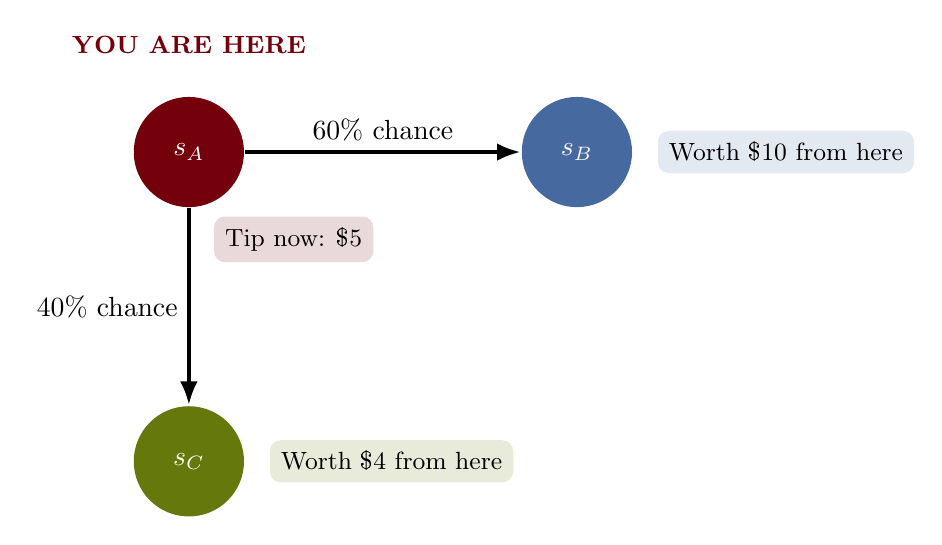
\begin{tikzpicture}[thick, node distance=3.5cm]
        % States
        \node[circle, fill=Garnet, text=white, minimum size=1.4cm] (A) {$s_A$};
        \node[circle, fill=SecondaryBlue, text=white, minimum size=1.4cm, right=of A] (B) {$s_B$};
        \node[circle, fill=SecondaryGreen, text=white, minimum size=1.4cm, below=2.5cm of A] (C) {$s_C$};

        % Arrows with probabilities
        \draw[-{Latex[length=3mm]}, line width=1.5pt] (A) -- node[above] {60\% chance} (B);
        \draw[-{Latex[length=3mm]}, line width=1.5pt] (A) -- node[left] {40\% chance} (C);

        % Value labels
        \node[right=0.3cm of B, font=\small, fill=SecondaryBlue!15, inner sep=4pt, rounded corners] {Worth \$10 from here};
        \node[right=0.3cm of C, font=\small, fill=SecondaryGreen!15, inner sep=4pt, rounded corners] {Worth \$4 from here};

        % Current state label
        \node[above=0.4cm of A, font=\small\bfseries, text=Garnet] {YOU ARE HERE};
        \node[below right=0.3cm and -0.2cm of A, font=\small, fill=Garnet!15, inner sep=4pt, rounded corners] {Tip now: \$5};
    \end{tikzpicture}
\end{document}
